\documentclass{l4proj}

%
%  Macro files
%  Originally from Frisch, Castagna, Benzaken
%  
%

%% Ornela
\newcommand{\abstr}[4]{\lambda_{({#1} , {#2})} {#3}.{#4}}
\newcommand{\semval}[2]{\sem{#1}_{\mathcal #2}}



\newif{\ifSHORT}
\newif{\ifLongVersion}
\newif{\ifWithRecords}
\newif{\ifWiths}

\newcommand{\possiblecut}[1]{{\color{black}#1}}   

\newcommand{\maincomment}[1]{%
  \ifMarginalComments{\mbox{}\\[1mm]$\Longrightarrow$\textsf{#1}\mbox{}\\[1mm]} \else {} \fi}

\newenvironment{mylist}{%
\begin{list}{$\bullet$}{\topsep2pt\parskip0pt\partopsep0pt\itemsep3pt\labelwidth10.5mm\labelsep3pt\leftmargin11mm}}%
{\end{list}}

%
%  unsemplice comando che mi dice la versione
%
\usepackage{calc}\newcounter{tempo}\setcounter{tempo}{\time}
\newcommand{\version}[1]{\mbox{}\\[-\baselineskip]%
   \raisebox{#1in}[0in][0in]{\makebox[\textwidth][c]{\rm\small \today:v.\thetempo}}}
\newcommand{\titlepageheader}[1]{\mbox{}\\[-\baselineskip]%
\raisebox{5.3in}[0in][0in]{\makebox[\textwidth][c]{\rm\small #1}}}
\newcommand{\duce}{$\mathbb{C}$Duce }
\newcommand{\cduce}{$\mathbb{C}$Duce }
\newcommand{\cdoge}{$\mathbb{C}$Doge }
\newcommand{\cpi}{$\mathbb{C}\pi$ }
\newcommand{\cobj}{$\mathbb{C}$Obj }
\newcommand{\sempi}{$\pi_\leq$}   % was semantic-$\pi${}}
\newcommand{\emptyl}{\mathsf{empty}}
%
% Daniele
%
% altri commandi
\newcommand{\wt}[1]{\widetilde{#1}}

\newcommand{\synrnd}{\mathbf{rnd}}
\newcommand{\synclass}{\mathbf{class} \ }
\newcommand{\syninterface}{\mathbf{interface} \ }
\newcommand{\synext}{\ \mathbf{extends }\ }
\newcommand{\synimpl}{\ \mathbf{implements}\ }
\newcommand{\synret}{\mathbf{return}\ }
\newcommand{\synthis}{\mathbf{this}}
\newcommand{\synsuper}{\mathbf{super}}
\newcommand{\synfinal}{\mathbf{final}}
\newcommand{\synnew}{\mathbf{new}\ }
\newcommand{\syndecl}[3]{\synclass #1 \synext #2\ \{#3\}}
\newcommand{\synidecl}[2]{\synclass #1 \synext #2\ }

\newcommand{\mmif}{\mathbf{if}}
\newcommand{\mmthen}{\mathbf{then}}
\newcommand{\mmelse}{\mathbf{else}}
\newcommand{\mmclass}{\mathbf{class}}
\newcommand{\mmnew}{\mathbf{new}}
\newcommand{\mmnull}{\mathbf{null}}
\newcommand{\mmextends}{\mathbf{extends}}
\newcommand{\mmint}{\mathbf{int}}
\newcommand{\mmreal}{\mathbf{real}}
\newcommand{\mmbool}{\mathbf{bool}}
\newcommand{\mmtrue}{\mathbf{true}}
\newcommand{\mmfalse}{\mathbf{false}}
\newcommand{\nname}{\mathbf{name}}
\newcommand{\mmreturn}{\mathbf{return}}
\newcommand{\mminstof}{\mathbf{instanceof}}
\newcommand{\mmtry}{\mathbf{try}}
\newcommand{\mmcatch}{\mathbf{catch}}
\newcommand{\mmthrow}{\mathbf{throw}}
\newcommand{\mmlet}{\mathbf{let}}
\newcommand{\mmin}{\mathbf{in}}
\newcommand{\nominal}{\mathbf{nominal}}

\newcommand{\naming}[1]{(#1)^\nname}
\newcommand{\type}{\mathit{type}}
\newcommand{\mbody}{\mathit{body}}
\newcommand{\judge}[2]{#1 \vdash #2}
\newif\ifmai\maifalse


\newcommand{\height}[1]{\hslash(#1)}%{\textit{height}(#1)}
%\DeclareMathOperator{\uparrowop}{\uparrow}
%\DeclareMathOperator{\downarrowop}{\downarrow}
%
% definition enum environment
%
\newenvironment{enum}{\begin{enumerate}\vspace{-5pt}\topsep0pt\parskip0pt\partopsep0pt\itemsep1pt}{\end{enumerate}\vspace{-5pt}}


%
%
\newcommand{\A}{{\cal A}}
\newcommand{\Norm}{{\cal N}}
\newcommand{\exten}{\mathbb E}
\newcommand{\extenf}{\mathbb{E}_f}
\newcommand{\atoms}{{\mathbb T}}
\newcommand{\myitem}{\mbox{}\\[.5mm]\hspace*{3.5mm}--~~}

\newcommand{\dead}{\textsf{0}}
%\newcommand{\mathbb}[1]{\Bbb{#1}}
%\newcommand{\llbracket}{[\![}
%\newcommand{\rrbracket}{]\!]}

\newcommand{\VAR}{\textit{Var}}
\newcommand{\zero}{\mathbf{0}}
\newcommand{\one}{\mathbf{1}}
%\newcommand{\qed}{\mbox{}\hfill\mbox{$\Box$}}
\newcommand{\bij}{\partial}
\newcommand{\para}{~~|~~}
\newcommand{\hasse}[1]{\xymatrix@R-1em@C-2em{#1}}

\newcommand{\todo}[1]{{\bf \underline{TODO:} #1}}
\newcommand{\ignore}[1]{}
\newcommand{\Is}{\colon\!\!\colon \!\!\!\!= }

\newcommand{\txtvee}{\text{\rm ~or~}}
\newcommand{\txtwedge}{\text{\rm ~and~}}

\newcommand{\dom}{\textit{dom}}

%\newcommand{\naturals}{\mathbb{N}}

% Op�rateurs math�matiques
\renewcommand{\P}{{\cal P}}
\newcommand{\Pf}{{\P_f}}
\newcommand{\compl}[2]{{\complement_{#2}} {#1}}
\newcommand{\egdef}{\stackrel{\textrm{\tiny def}}{=}}
\newcommand{\segdef}{\!\!\!\stackrel{\textrm{\tiny def}}{=}\!\!\!}
\renewcommand{\subset}{\subseteq}
\renewcommand{\emptyset}{\varnothing}

\newcommand{\cX}{{\cal X}}

% Les univers
\newcommand{\ubasic}{{\text{\bf basic}}}
\newcommand{\urec}{{\text{\bf rec}}}
\newcommand{\ufun}{{\text{\bf fun}}}

% Basic types
\newcommand{\btypes}{{\mathbb B}}
\newcommand{\semb}[1]{{\cal B} {\llbracket #1 \rrbracket}}
\newcommand{\Types}{\textbf{Types}}
% Les mod�les
\newcommand{\domaine}{{\cal D}}
%\newcommand{\univ}{{\cal U}}
\newcommand{\domwr}{\domaine_\Omega}
\newcommand{\stdmod}{{\cal U}}
\newcommand{\stdmodwr}{{\cal U}_\Omega}
\newcommand{\sem}[1]{{\llbracket #1 \rrbracket}}
\newcommand{\esem}[1]{{\mathbb E}\left( #1 \right)}
\newcommand{\esemd}[1]{{\mathbb E}$D$}
\newcommand{\esemp}[1]{{\cal E}\llparenthesis #1 \rrparenthesis}
\newcommand{\tsem}[1]{\llparenthesis #1 \rrparenthesis}
%\newcommand{\semv}[1]{{\mathbb V}{\llbracket #1 \rrbracket}}


% Les types
\newcommand{\functor}{{\mathbb T}}
\newcommand{\syntypes}{{\mathcal{T}}}
\newcommand{\atomtypes}{\textit{A\/}}%{\syntypes^\circ}
\newcommand{\synatoms}{{\mathcal A}}
\newcommand{\synprod}{\pmb{\times}}
\newcommand{\synarrow}{\pmb{\rightarrow}}
\newcommand{\synneg}{\pmb{\neg}}
\newcommand{\synvee}{\pmb{\vee}}
\newcommand{\synwedge}{\pmb{\wedge}}
\newcommand{\syndiff}{\pmb{\backslash}}
\newcommand{\syncap}{\operatornamewithlimits{\pmb{\bigwedge}}}
\newcommand{\syncup}{\operatornamewithlimits{\pmb{\bigvee}}}
\newcommand{\socle}[1]{\beth(#1)}
\newcommand{\appl}{\bullet}
\newcommand{\synch}[2]{\textit{ch}^{#1}\!(#2)}
\newcommand{\synchan}[1]{\textit{ch}(#1)}
\newcommand{\synchanK}{\textit{ch}}
\newcommand{\synchanout}[1]{\textit{ch}^{\!\textbf{--}\!\!}(#1)}
\newcommand{\synchanin}[1]{\textit{ch}^+(#1)}

%blackboardbold types
\def\bbbone{{\mathchoice {\rm 1\mskip-4mu l} {\rm 1\mskip-4.5mu l}
          {\rm 1\mskip-4.5mu l} {\rm 1\mskip-5mu l}}}
\newcommand{\synnatone}{\bbbone}
\newcommand{\synnatk}{\Bbbk}
\newcommand{\synnat}[1]{\mathbb{#1}}

% Les motifs
\newcommand{\pator}[2]{#1 \pmb{|} #2}
\newcommand{\patand}[2]{#1 \pmb{\wedge} #2}
%\newcommand{\patleft}[1]{\pmb{(}#1\pmb{,\_)}}
%\newcommand{\patright}[1]{\pmb{(\_,}#1\pmb{)}}
\newcommand{\patcst}[2]{\pmb{(}#1\pmb{:=}#2\pmb{)}}
\newcommand{\patpair}[2]{\pmb{(}#1\pmb{,}#2\pmb{)}}

% Filtrage
\newcommand{\erreur}{\Omega}
\newcommand{\accept}[1]{\pmb{\lbag} #1 \pmb{\rbag}}
\newcommand{\acceptd}[1]{\pmb{\lfloor} #1 \pmb{\rfloor}}
\newcommand{\semaccept}[1]{\Lbag #1 \Rbag}
\newcommand{\filter}[2]{({#1}/{#2})}%{ ({#1} \Downarrow {#2}) }
\newcommand{\semfilter}[2]{ ({#1} \downarrow {#2}) }


% Symboles du langage
%\newcommand{\myarrow}{\Pisymbol{cmt}{61}\Pisymbol{pcr}{62}}%
\newcommand{\myarrow}{\!\!\boldsymbol{\Rightarrow}\!\!} %\texttt{\char61\char62\relax}}
\newcommand{\mybar}{\texttt{|}}%
\newcommand{\motifs}{\mathbb{P}}
\newcommand{\vars}{\mathbb{V}}
\newcommand{\consts}{\mathbb{C}}
\newcommand{\exprs}{{\mathbb E}}
\newcommand{\expr}{{e}}
\newcommand{\pat}{{\tt p}}
\newcommand{\const}{{n}}
\newcommand{\op}{{o}}
\newcommand{\ops}{{\mathbb O}}
\newcommand{\valeurs}{{\cal V}}
\newcommand{\values}{\valeurs}
\newcommand{\blpar}{\boldsymbol{(}}
\newcommand{\brpar}{\boldsymbol{)}}
\newcommand{\match}[5]{\mathtt{match~} #1 \mathtt{~with~} #2 \myarrow #3 \mybar
  #4 \myarrow #5}
\newcommand{\typecase}[5]{\mathtt{typecase~} #1 \mathtt{~with~} (#2 :
  #3) \myarrow #4 \mybar (#2 : \synneg #3) \myarrow #5}
\newcommand{\typec}[5]{\texttt{(} #3=#1\pmb{\in}#2\texttt{)}\pmb{?}#4\texttt{{:}}#5}
\newcommand{\genabstraction}[3]{\abstr{f}{#1}{#2}{#3}}
%\newcommand{\abstr}[4]{\boldsymbol{\mu} #1^{\blpar #2 \brpar}\blpar #3 \brpar \boldsymbol{.}#4}
\newcommand{\stdmatch}{\match{\expr}{p_1}{\expr_1}{p_2}{\expr_2}}
\newcommand{\exprpair}[2]{\blpar #1 \boldsymbol{,} #2 \brpar}
\newcommand{\exprop}[2]{#1 \blpar #2 \brpar}

% S�mantique op�rationnelle
%\newcommand{\wrong}{\mbox{\bf wrong}}
\newcommand{\wrong}{\Omega}
%\newcommand{\reject}{\mbox{\bf reject}}
%\newcommand{\apply}{{\tt apply}}


% Enregistrements
\newcommand{\domdef}[1]{\text{Def}(#1)}
\newcommand{\labels}{{\cal L}}
\newcommand{\urecord}{{\text{\bf record}}}
\newcommand{\trec}[2]{\pmb{[} #1 : #2 \pmb{]}}
\newcommand{\tsupp}[1]{\text{\bf S}(#1)}
%\newcommand{\supp}[1]{\text{Supp}(#1)}
\newcommand{\patrec}[2]{\{ #1 : #2\}}
\newcommand{\Iff}{\Longleftrightarrow}
\newcommand{\reff}{\mathtt{ref}\,}
\newcommand{\lazy}{\mathtt{lazy}\,}


% Th�or�mes ...
%\newtheorem{theorem}{Theorem}[section]
%\newtheorem{lemma}[theorem]{Lemma}
%\newtheorem{proposition}[theorem]{Proposition}
%\newtheorem{corollary}[theorem]{Corollary}
%\newtheorem{definition}[theorem]{Definition}
%\newtheorem{condition}{Condition}
%\newenvironment{definition}{\begin{defn}}{\qed\end{defn}}
%\newtheorem{definition}[theorem]{Definition}
%\newtheorem{property}[theorem]{Property}
%\newtheorem{convention}[theorem]{Convention}
%\newtheorem{remark}[theorem]{Remark}
%\renewenvironment{proof}{{\sl Proof}:}{\qed}

\usepackage{amsmath, amssymb}

\begin{document}

%===================================================================================================

\title{Boolean types and semantic subtyping for Featherweight Java}
\author{Artem Usov}
\date{January 18, 2020}

\maketitle

%===================================================================================================

\begin{abstract}
    Every abstract follows a similar pattern. Motivate; set aims; describe work; explain results.
    \vskip 0.5em
    ``XYZ is bad. This project investigated ABC to determine if it was better.
    ABC used XXX and YYY to implement ZZZ. This is particularly interesting as XXX and YYY have
    never been used together. It was found that
    ABC was 20\% better than XYZ, though it caused rabies in half of subjects.''
\end{abstract}

%===================================================================================================

\def\consentname {Artem Usov}
\def\consentdate {19 January 2020}
\educationalconsent

%===================================================================================================

\tableofcontents

%===================================================================================================

\chapter{Introduction}

\pagenumbering{arabic}

\section{End goal of programming}

The end goal in all programming projects is to create a solution to the task at hand that exactly solves the initially defined problem and performs exactly as expected by the programmer.
However, this very rarely actually happens.

On the one hand, this is often because the original problem is not statically defined.
If it is a solution for an external client, then their requirements and needs will change over time, or similarly the needs and wants of the users using this project can also change.
This means the project needs to be adapted over time.
On the other hand, and almost always much less evident, is that programs do not work exactly as the programmer imagines them to work.

These are in general called \emph{bugs} in a program, and have become more and more common as projects have become more complex compared to the early days of computing and the underlying hardware we work on has also become more complex.
Therefore in both academia and industry there have been great efforts over the years to create tools that allow us to decrease the amount of bugs in our programs and increase our productivity.

\subsection{Static Code Analysis}

One area of great effort has been in the development of static code analysis tools.
Some of these exist integrated into the language itself such as with Spark \citep{Carre1990}.
Spark is a formally defined language based on the Ada \citep{Ada1979} language intended for the development of high integrity software such as flight control systems.
Others exist as separate, well-known tools that exist alongside the language such as the Clang analysis tools for C and C++ \citep{kremenek2008}.

Whilst they are not necessarily needed to write correct programs, these tools have quickly become industry standards for maintaining a level of correctness within codebases and avoiding typical programming errors.

\subsection{Into Static Analysis}

Underlying all of the previously mentioned static code analysis tools, is their use of the \emph{type system} of the language.
Type systems at their most basic work by assigning types to various constructs of a program so that incompatible types cannot be used.

For example, one common area of error in C code that the Clang tools warn about is implicit conversions, where the value of an expression is a different type from the one expected, such as the use of a floating point number where an integer is expected.
The C language will implicitly convert the value to an integer, however this can cause unexpected behaviour, unbeknownst to the programmer.
Whilst being inconvenient, this conversion needs to happen as the type system of the language dictates that you cannot use any other type other than an integer where an integer is expected.

\section{Varying Type Systems}

The effectiveness of static analysis tools and more generally the \emph{safety} and \emph{expressivity} of a programming language therefore depends on the type system that is used.
Type systems have evolved from the relatively simple systems in languages like C to more complex ones such as in Java where there are custom object types and subtyping relations where types can be substituted for one another.

More modern advances in type systems include the use of linear types in the Cyclone \citep{grossman2002} language that allow us to more naturally and logically define finite state machines.
There also exist other new developments in type systems such as Boolean types which are explored in this paper.

\section{Goals of this Project}

In this section, the issues and aims of this paper are presented.

\subsection{Problem Statement}

The typical hierarchical subtyping definitions in Java quite often restrict and complicate the logic that the programmer wants to implement.
These problems come up particularly often when working with legacy code that has incorrectly defined abstractions in its classes.
This therefore leads to less understandable and less maintainable code that could cause problems in the future.

\subsection{Aims}

The aim of this project is to implement a new programming language, which we further call Semantic Featherweight Java (SFJ), which uses a new proposed type system consisting of boolean types and a semantic subtyping algorithm.
This project aims to transform the mathematical definition of such a type system into an actual software implementation, solving the issues encountered doing so.
The language should be able to illustrate the improved solutions to the common example problems encountered in a language without these features such as Java.
Furthermore, the language will be evaluated so see whether these additional language features are intuitive to use.

\section{Dissertation Outline}

The dissertation is structured into seven chapters as follow:

\begin{itemize}
    \item
          \textbf{Chapter 2} provides background about type systems and Featherweight Java, the language on top of which the new type system is implemented.
          We also discuss some existing work on semantic type systems and boolean types.
    \item
          \textbf{Chapter 3} TODO
    \item
          \textbf{Chapter 4} TODO
    \item
          \textbf{Chapter 5} TODO
    \item
          \textbf{Chapter 6} contains details about the evaluation method, evaluation results and analysis of results.
    \item
          Finally \textbf{chapter 7} concludes the dissertation with a summary of the important results.
\end{itemize}

%===================================================================================================

\chapter{Background}

In this chapter, we define and explore type systems and the different ways they can be defined. We especially explore the semantic method of defining a type system and explore the benefits and challenges that it brings. We also discuss the tools that were used in this project and the related work that has already been done with boolean types or semantic type systems.

\section{Type Systems}

In all modern programming languages, a \emph{type system} is arguably the main way that incorrect behaviour in a program is reduced by preventing the occurrence of \emph{type errors}.
A possible definition of a type system is given by \citet{Pierce2002} as:

\emph{A type system is a tractable syntactic method for proving the absence of certain program behaviors by classifying phrases according to the kinds of values they compute.}

A type error is defined by \citet{wright1994} as:

\emph{The use of a function on arguments for which it is not defined, and the attempted application of a non-function.}

Most importantly, we want to emphasize from the first definition that in a type system, we aim to classify phrases in our language into a specific \emph{type}.
Then, using the type system, we can check that the types of the arguments given to any operation are always correct, thus avoiding a type error.

For example, taking the addition operation which takes two arguments of the number type, then given the arguments $42$ and $2 + 2$, we know they both hold or compute a number type and so there is guaranteed to be no type error.
Conversely, given the arguments $42$ and the boolean value $true$, they are not both a number type and so cause a type error.
We therefore avoid unexpected bad run-time behaviour and instead find these problems before even running the program.

However what the first definition is missing is that it defines a type system to be solely a syntactic method, in which the system is defined as a list of formal deduction rules.
The syntactic approach is certainly by far the most common approach for a type system, but there does exist an alternative method in the semantic approach.
\citet{Frisch2002} describe the semantic approach as instead starting with a model of the language and all the possible values in the language and defining an interpretation of types as subsets of values the model.

For example, given a language with a model $D$:

\begin{equation*}
    D = \left[ a + bi \mid a, b \in \mathbb{R}\right]
\end{equation*}

we can define the types \emph{int}, \emph{real} and \emph{complex} as subsets of the values in $D$ corresponding to their usual mathematical definitions.

Such as model comes with several advantages.
For example, given two types $s$ and $t$, which represent subsets of values in the model, when $s \subseteq t$ does not hold, it is possible to exhibit an element of the model which is in the interpretation of type $s$ and not $t$.
This can then be used to show more informative error messages to the programmer as shown by \citet{Castagna2005}, such as showing which value in $s$ is causing the equality not to hold.
Secondly the set based approach to the type system leads itself to able to incorporate boolean operators into its types easily.
However due to being a more technical approach, such as the non-triviality of defining the interpretation of types as subsets of a model as discussed below, the semantic method has received less attention than syntactic methods.

The first problem we encounter in the semantic approach is that in such a model, $t_{1}$ is a subtype of $t_{2}$ if all the $t_{1}$-values are also $t_{2}$-values, i.e. the equality $t_{1} \subseteq t_{2}$ holds.
However, in this way, subtyping is defined by relying on the notion of well-typed values; hence, we need the typing relation to able to type values; but the typing rules require a subtyping relation to be fully defined.
So, there is a circularity in our definition, as demonstrated in Figure \ref{fig:circ}.

To solve this problem, we follow the framework defined by \citet{Frisch2008}.
The general idea of the framework is that we first extend the types in the language with \emph{Boolean Combinators}: union $\lor$, intersection $\land$ and negation $\neg$ to give a type algebra $\tau$.
We can then define an abstract model $\beta$ with a interpretation function $[\![ ]\!]_{\beta} : \tau \to \rho(\beta)$ (where $\rho(\beta)$ is the power-set of $\beta$).
This model must capture the meaning of each type but also interprets the combinators in a set-theoretic way, such as $[\![s \land t]\!]_{\beta} = [\![s]\!]_{\beta} \cap [\![t]\!]_{\beta}$ etc.
This model then induces the following subtyping relation:

\begin{equation*}
    s \leq_{\beta} t \iff [\![s]\!]_{\beta} \subseteq [\![t]\!]_{\beta}
\end{equation*}

and we can therefore define the typing rules.

Separately, now that we have typing rules, we can define a new interpretation of types based on values $[\![t]\!]_{\mathrm{v}} = \left\{\mathrm{v} \in V \mid \: \vdash_{\beta} \mathrm{v} : t \right\}$ and then define a ``new''subtyping relation as above:

\begin{equation*}
    s \leq_{\mathrm{v}} t \iff [\![s]\!]_{\mathrm{v}} \subseteq [\![t]\!]_{\mathrm{v}}
\end{equation*}

While these may be different relations, if the models are chosen carefully such that:
\begin{equation*}
    s \leq_{\beta} t \iff s \leq_{\nu} t,
\end{equation*}

then these subtyping relations coincide and this closes the circularity.

\begin{figure}
    \centering
    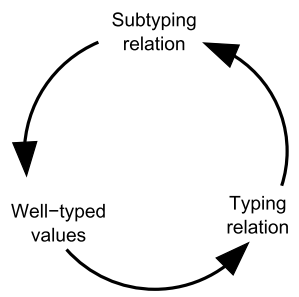
\includegraphics[width=0.4\linewidth]{images/circularity.PNG}
    \caption{Circularity in the semantic subtyping definition \citep{Castagna2005}}
    \label{fig:circ}
\end{figure}

\section{Featherweight Java}

The syntax of SFJ is exactly that of Featherweight Java (FJ) \citep{Igarashi1999}, with only the associated type system being different.
FJ is closely related to Java, with a key simplification in the removal of assignment operators.
All fields of an object cannot be changed after initialisation and all methods are pure functions.
While this restricts FJ to what is essentially a functional fragment of Java, it is still fully computationally complete.
SFJ was intentionally based on FJ instead of the full Java language because features such as concurrency and reflection are orthogonal to the purpose of demonstrating the implementation of our novel semantic type system.

\paragraph{On multimethods}
Since FJ is a core language, some features of the full Java are removed: overloading methods is one of them.
In our framework, leveraging the expressivity of boolean connectives and semantic subtyping, many of these features, and language constructs, e.g., lists, are restored: overloading methods is one of them. We can thus model \emph{multimethods} \citep{BC97}, which according to the authors is ``\emph{very clean and easy to understand [...] it would be the best solution for a brand new language}".
As an example \citet{Dardha2013,Dardha2017}, consider the following class declarations:
$$
    \begin{array}{ll}
        \syndecl{A}{\mathit{Object}} {
         &
            \qquad
            \syndecl{B}{A} {
                \\
                \qquad\quad \mathbf{int}\ \mathit{length}\ (\mathbf{string}\ s)\{\ \ldots\ \}\qquad
         &
                \qquad\qquad\quad \mathbf{int}\ \mathit{length}\ (\mathbf{int}\ n)\{\ \ldots\ \}
                \\
            }
         &
            \qquad }
    \end{array}
$$
Method {\it length} has type $\mathbf{string} \rightarrow \mathbf{int}$ in $A$. However, in $B$ it has type $(\mathbf{string} \rightarrow \mathbf{int}) \synwedge (\mathbf{int} \rightarrow \mathbf{int})$,
which can be simplified as $(\mathbf{string} \synvee \mathbf{int}) \rightarrow \mathbf{int}$.


\section{Tools}

The type system of FSJ was built using ANTLR \citep{parr2013} to define the grammar of the language and automatically create a parser for this grammar rather than having to create one by hand, which made the initial development process much quicker.
It accepts a grammar using Extended Backus-Naur Form (EBNF) \footnote{See ISO/IEC 14977 for reference, although it is not the standard used in the examples} notation to create ANTLR rules which are a list of productions or alternatives.
A general form of a rule is as follow:

$$
    \begin{array}{llll}
        rule & : & alternative_{1}
        \\
             & | & alternative_{2}
        \\
             &   & \vdots
        \\
             & | & alternative_{n}
        \\
             & ; &
    \end{array}
$$

Each alternative production in a rule can itself be a list of elements, where an element can be another rule or just a terminating token.
Since we are using EBNF notation, we can also use \emph{*} and \emph{?} to respectively signify repeated and conditional elements in a production.
We can also use $|$ to give several alternatives for a single element.
We show an excerpt taken from the SFJ grammar as an example:

$$
    \begin{array}{llll}
        expression     & : & \mbox{primExpression ( (PLUS | MINUS | DIV | MULT) primExpression)?}
        \\
                       & ;
        \\
        \\
        primExpression & : & \mbox{NUMBER}
        \\
                       & | & \mbox{TRUE}
        \\
                       & ; &
        \\
        \\
        TRUE           & : & \mbox{'true'}
        \\
                       & ; &
        \\
        \\
        NUMBER         & : & \mbox{DIGIT (DIGIT)*}
        \\
                       & ; &
        \\
        \\
        DIGIT          & : & '0'..'9'
        \\
                       & ; &
    \end{array}
$$

\section{Related Work}
The closest similar area of research would likely be the work on $\mathbb{C}$Duce
\citep{Benzaken2003}, which is xalso a functional language with a semantic type system designed for
working with XML documents and a continuation of the work on XDuce \citep{Hosoya2003}. The language
extended XDuce by introducing less XML specific types such as records, boolean connectives and arrow
types. This therefore makes it similar to (\textit{TODO reword}) our language in that a class-based
semantic type system is a combination of the $\mathbb{C}$Duce record types with arrow types
\textit{(fields and methods)}

Our work and the work on $\mathbb{C}$Duce follow the functional style of $\lambda$-calculus,
whereas the work by \citet{Castagna2008} extends $\pi$-calculus with semantic subtyping.
(\textit{TODO reword}) Similar work to ours creating an implementation for this would result in a
Golang-like \footnote{https://golang.org/} like language, creating a concurrency-focused language with more
intuitive types. The paper found that it was required to be able to decide and resolve the atomicy,
that is whether the only proper subtype is the empty type, of types in order to decide the subtyping
relation, and observes that this same problem appears in $\lambda$-calculus and any other
semantic-based system, for which we will show where we encountered this problem further in this
paper.

%===================================================================================================

% \chapter{Analysis/Requirements}
% What is the problem that you want to solve, and how did you arrive at it?
% \section{Guidance}
% Make it clear how you derived the constrained form of your problem via a clear and logical process.

%===================================================================================================
\chapter{SFJ: Design and Implementation}

\section{Syntax}

\subsection{Syntax of Types}

\label{sec:design}
The syntax of types is given by the following grammar \citep{Dardha2013,Dardha2017}:
$$
    \begin{array}{llll}
        \tau   & ::=                                       & \alpha \ |\ \mu
               & \mbox{{\em Type term}}
        \\
        \alpha & ::=                                       & \zero \ |\ \btypes \ |\ [\wt{l:\tau}] \ |\ \alpha \ \bf{and}\ \alpha \ |\ \bf{not}\ \alpha
        \qquad
               & \mbox{{\em Object type} ($\alpha $-type)}
        \\
        \mu    & ::=                                       & \alpha \to \alpha \ |\ \mu \ \bf{and}\ \mu \ |\ \bf{not}\ \mu
               & \mbox{{\em Method type} ($\mu $-type)}
    \end{array}
$$

$\alpha$-types are used to type fields and $\mu$-types are used to type methods.
Type $\zero$ is the empty type.
Type $\btypes$ denotes the \emph{basic} types, such as integers, booleans, etc.
    {Record} types $[\wt{l:\tau}]$, where $\wt l$ is a sequence of disjoint labels are used to type objects.
Arrow types $\alpha \to \alpha$ are used to type methods.
The boolean types using ${and}$ and ${not}$ have their expected set-theoretic meanings, and ${or}$ is obtained by their combination.\\

\subsection{Syntax of Terms}

The syntax of terms is given by the following grammar and is based on the standard syntax of terms in FJ \cite{Igarashi1999,Dardha2013,Dardha2017}.
We assume an infinite countable set of names, with some special names: $\mathit{Object}$ indicates the root class, $\synthis$  indicates the current and $\synsuper$ indicates the parent object.
We let  $A, B, C, \ldots$ range over classes; $a, b, \ldots$ over fields; $m, n, \ldots$ over methods and $x, y, z, \ldots$ range over variables.
Constants $c$ range over an infinite countable set $\mathcal{K}$.

\begin{align*}
     & \mbox{\textit{Class declaration}}  & L \; ::= \; & \syndecl{C}{C}{\wt{\alpha \ a};\ K; \ \wt{M}\ }                         \\
     & \mbox{\textit{Constructor}}        & K \;::=\;   & C\ (\wt{\alpha\ x})\ \{\ \synsuper(\wt{x});\ \wt{\synthis.a}=\wt{x}; \} \\
     & \mbox{\textit{Method declaration}} & M \; ::= \; & \alpha \ m\ (\alpha \ x)\ \{\ \synret e; \}                             \\
     & \mbox{\textit{Expressions}}        & e \; ::=\;  & x\ |\  c\ |\ e.a\ |\ e.m(e) \ | \ \synnew C(\wt{e})
\end{align*}

A {program} $(\wt{L}, e)$ is a pair of a sequence of class declarations $\wt L$, giving rise to a class hierarchy as specified by the inheritance relation, and an expression $e$ to be evaluated.
%
A class declaration $L$ specifies the name of the class, the name of the parent class it extends, its typed fields , the constructor $K$ and its method declarations $M$.
The constructor $K$ initializes the fields of the object by assigning values to the fields inherited by the super-class and to the fields declared in the current \textbf{this} class.
%
A method declaration $M$ specifies the signature of the method, namely the return type, the method name and the formal parameter as well as the body of the method.
Notice that in our theoretical development we use unary methods, without loss of generality: tuples of arguments can be modelled by an object that instantiates a ``special''class containing as fields all the needed arguments.
Expressions $e$ include variables, constants, field accesses, method invocations and object creations.

%===================================================================================================

\chapter{Implementation}

What did you do to implement this idea, and what technical achievements did you make?

\section{Guidance}
You can't talk about everything. Cover the high level first, then cover important, relevant or impressive details.

\section{General points}

These points apply to the whole dissertation, not just this chapter.

\subsection{Figures}

\emph{Always} refer to figures included, like Figure \ref{fig:relu}, in the body of the text. Include full, explanatory captions and make sure the figures look good on the page.
You may include multiple figures in one float, as in Figure, using \texttt{subcaption}, which is enabled in the template.

\subsection{Equations}

Equations should be typeset correctly and precisely. Make sure you get parenthesis sizing correct, and punctuate equations correctly
(the comma is important and goes \textit{inside} the equation block). Explain any symbols used clearly if not defined earlier.

For example, we might define:
\begin{equation}
    \hat{f}(\xi) = \frac{1}{2}\left[ \int_{-\infty}^{\infty} f(x) e^{2\pi i x \xi} \right],
\end{equation}
where $\hat{f}(\xi)$ is the Fourier transform of the time domain signal $f(x)$.

\subsection{Algorithms}

Algorithms can be set using \texttt{algorithm2e}, as in Algorithm.

\subsection{Tables}

If you need to include tables, like Table , use a tool like https://www.tablesgenerator.com/ to generate the table as it is extremely tedious otherwise.

\subsection{Code}

Avoid putting large blocks of code in the report (more than a page in one block, for example). Use syntax highlighting if possible, as in Listing.

%===================================================================================================

\chapter{Evaluation}
How good is your solution? How well did you solve the general problem, and what evidence do you have to support that?

\section{Guidance}

\begin{itemize}
    \item
          Ask specific questions that address the general problem.
    \item
          Answer them with precise evidence (graphs, numbers, statistical
          analysis, qualitative analysis).
    \item
          Be fair and be scientific.
    \item
          The key thing is to show that you know how to evaluate your work, not
          that your work is the most amazing product ever.
\end{itemize}

\section{Evidence}
Make sure you present your evidence well. Use appropriate visualisations, reporting techniques and statistical analysis, as appropriate.

If you visualise, follow the basic rules, as illustrated in Figure:
\begin{itemize}
    \item Label everything correctly (axis, title, units).
    \item Caption thoroughly.
    \item Reference in text.
    \item \textbf{Include appropriate display of uncertainty (e.g. error bars, Box plot)}
    \item Minimize clutter.
\end{itemize}

See the file \texttt{guide\_to\_visualising.pdf} for further information and guidance.


%===================================================================================================

\chapter{Conclusion}

Summarise the whole project for a lazy reader who didn't read the rest (e.g. a prize-awarding committee).

\section{Guidance}
\begin{itemize}
    \item
          Summarise briefly and fairly.
    \item
          You should be addressing the general problem you introduced in the
          Introduction.
    \item
          Include summary of concrete results (``the new compiler ran 2x
          faster'')
    \item
          Indicate what future work could be done, but remember: \textbf{you
              won't get credit for things you haven't done}.
\end{itemize}

%===================================================================================================

%  APPENDICES

\begin{appendices}


    \chapter{SFJ ANTLR Grammar}

    \begin{lstlisting}
        grammar jsf;

        @header{
        package jsf;
        }

        program
                :       classDecl* expression EOF
                ;

        classDecl
                :   CLASS classlbl=ID (EXTEND extendlbl=ID)? LBRAC
                        fieldDecl* constructorDecl methodDecl*
                    RBRAC
                ;

        fieldDecl
                :       type ID SEMI
                ;

        constructorDecl
                :       constructorname=ID LPAR (type ID (COMMA type ID)*)? RPAR LBRAC
                            superDecl
                            fieldAssignment*
                        RBRAC
                ;

        superDecl
                :       SUPER LPAR (ID (COMMA ID)*)? RPAR SEMI
                ;

        fieldAssignment
                :       THIS DOT field=ID EQ parameter=ID SEMI
                ;

        methodDecl
                :       returntype=type name=ID LPAR (paramtype=methodType paramname=ID)? RPAR LBRAC
                            RETURN expression SEMI
                        RBRAC
                ;

        expression
                :       e1=primExpression
                            (op=(PLUS | MINUS | DIV | MULT) e2=primExpression)?
                ;

        primExpression
                :       NUMBER
                |       DECIMAL
                |       TRUE
                |       FALSE
                |       ID
                |       THIS
                |       primExpression DOT ID
                |       primExpression DOT ID LPAR (expression)? RPAR
                |       NEW ID LPAR (expression (COMMA expression)*)? RPAR
                ;

        type
                :       basicType
                |       ID
                |       NOT classlbl=type
                |       LPAR type1=type bool=(AND | OR) type2=type RPAR
                ;

        basicType
                :       BYTE | INT | LONG | FLOAT | DOUBLE | CHAR | BOOL
                ;

        methodType
                : type
                | LPAR (NOT)? ID COLON param=type ARROW returnType=type RPAR
                ;


        BYTE    :       'byte'                      ;
        INT     :       'int'                       ;
        LONG    :       'long'                      ;
        FLOAT   :       'float'                     ;
        DOUBLE  :       'double'                    ;
        CHAR    :       'char'                      ;
        BOOL    :       'bool'                      ;

        TRUE    :       'true'                      ;
        FALSE   :       'false'                     ;

        AND     :       'and'                       ;
        OR      :       'or'                        ;
        NOT     :       'not'                       ;

        CLASS   :       'class'                     ;
        SUPER   :       'super'                     ;
        EXTEND  :       'extends'                   ;
        THIS    :       'this'                      ;
        RETURN  :       'return'                    ;
        NEW     :       'new'                       ;

        LPAR    :       '('                         ;
        RPAR    :       ')'                         ;
        LBRAC   :       '{'                         ;
        RBRAC   :       '}'                         ;
        EQ      :       '='                         ;
        PLUS    :       '+'                         ;
        MINUS   :       '-'                         ;
        DIV     :       '/'                         ;
        MULT    :       '*'                         ;
        COMMA   :       ','                         ;
        DOT     :       '.'                         ;
        SEMI    :       ';'                         ;
        COLON   :       ':'                         ;
        ARROW   :       '->'                        ;

        ID      :       LETTER (LETTER | DIGIT)*    ;
        NUMBER  :       DIGIT (DIGIT)*              ;
        DECIMAL :       DIGIT DOT (DIGIT)*          ;
        SPACE   :       (' ' | '\t')+   -> skip     ;
        EOL     :       '\r'? '\n'      -> skip     ;
        EMPTY   :       'EMPTY'                     ;

        fragment LETTER :   'a'..'z' | 'A'..'Z'     ;
        fragment DIGIT  :   '0'..'9'                ;
    \end{lstlisting}

    \chapter{TODO}

\end{appendices}

%===================================================================================================

\bibliographystyle{abbrvnat}

\bibliography{l4proj}

\end{document}
